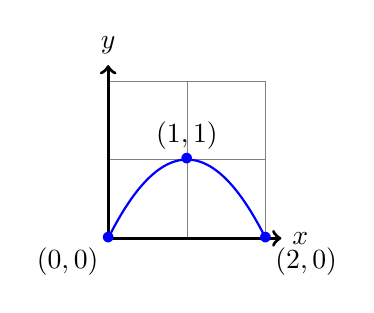
\begin{tikzpicture}[domain=0:2]
  %% \def\a{-2.45}
  %% \def\b{4.9}
  %% \def\c{0}
  \def\a{-1}
  \def\b{2}
  \def\c{0}
  %% The coordinates for the vertex are both integers.
  %% Drop the decimal part.
  \pgfmathsetmacro\h{int(-\b/(2*\a))}
  \pgfmathsetmacro\k{int(\a * \h^2 + \b * \h + \c)}

  \coordinate (V) at (\h,\k);
  
  \draw[very thin,color=gray] (0,0) grid (2,2);

  \draw[very thick,->] (0,0) -- (2.2,0) node[right] {$x$};
  \draw[very thick,->] (0,0) -- (0,2.2) node[above] {$y$};

  \draw [color=blue,thick] plot[smooth,samples=500] (\x,\a * \x^2 + \b * \x + \c);

  \node [blue] at (0,0) {$\bullet$};
  \node [below left] at (0,0) {$(0,0)$};
  
  \node [blue] at (2,0) {$\bullet$};
  \node [below right] at (2,0) {$(2,0)$};

  \node [blue] at (V) {$\bullet$};
  \node [above] at (V) {($\h,\k)$};
\end{tikzpicture}
